\chapter{Related Work}
\label{Chapter-Related-Work}
% tf and tff?
\section{Training Dataset}
The training dataset is the most important element of the training process, as ML models directly extract knowledge from it. Regardless of the training algorithm, using inadequate data can only result in underperforming models. A well-known adage still holds brutally true when it comes to training data for ML: garbage in, garbage out.

In the context of this work, the Fashion-MNIST \cite{fashion_mnist} dataset is utilized. It consists of 28 \(\times\) 28 grayscale images of 70,000 fashion items from 10 equally sized categories, split into a training set of 60,000 images and a testing set of 10,000 images. It is designed as a direct drop-in replacement of the original MNIST dataset \cite{digits_mnist} that provides a more challenging classification problem.

The major factor of its popularity is its small size which enables DL researchers to swiftly prototype and test their algorithms. Furthermore, it is highly accessible due to its strait-forward encoding and its permissive license. Finally, DL frameworks (e.g TensorFlow) provide auxiliary functions and convenient examples that use it right out of the box, makes it highly compelling.

\begin{figure}[H]
    \centering
        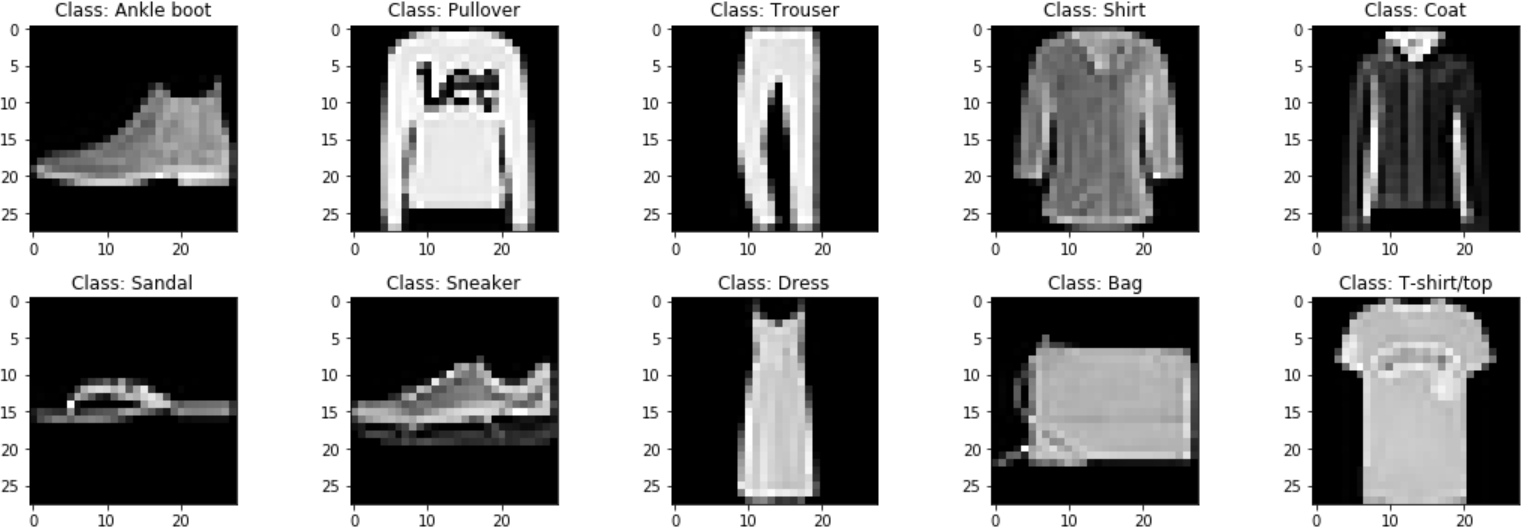
\includegraphics[width=0.9\textwidth]{Images/Examples_Fashion_MNIST.png}
        \decoRule
        \caption[Examples of Fashion MNIST Dataset]{Examples of Fashion MNIST Dataset: \href{https://www.bouvet.no/bouvet-deler/understanding-convolutional-neural-networks-part-2}{URL}.}
        \label{fig:Fashion_MNIST_dataset}
\end{figure}


\section{ANN architectures}
Any DL model that can be trained locally should be possible to be trained in FL, since FL is essentially another DL training method. To demonstate that the FL impementation in this work is accurate, multiple models of different architectures have been implemented and incorporated into the FL training loop. 

\subsection{LeNet-5}
LeNet-5 \cite{LeNet}, one of the first CNNs to describe its fundamental form, was proposed in 1989. Its original use was for handwritten digit recognition, a task in which it performed greatly and piqued academics' interest in the development and use of ANNs. It possesses the fundamental building blocks of CNNs, interconnected convolutional and pooling layers, followed by fully connected layers. Across all these layers it uses the tanh activation function, and to make the computation less difficult maintains sparse connections between them.

\subsection{AlexNet}
AlexNet \cite{Alexnet} is a CNN architecture designed to compete in the ImageNet Large Scale Visual Recognition Challenge of 2012. The depth of the network's model, five convolutional layers, some of which were followed by max-pooling layers, and then three fully connected layers, allowed it to outperform its competition in terms of accuracy. Furthermore, it used the non-saturating ReLU activation function, which shows better performance than prior activation functions like tanh.

Training such a large network on a CPU, which was the standard at that time, is computationally prohibitive, but was made possible by training it on graphics processing units (GPUs). That novelty spurred huge interest in CNNs and training them with accelerators, making it one of the most influential ANN architectures.

\begin{figure}[H]
    \centering
        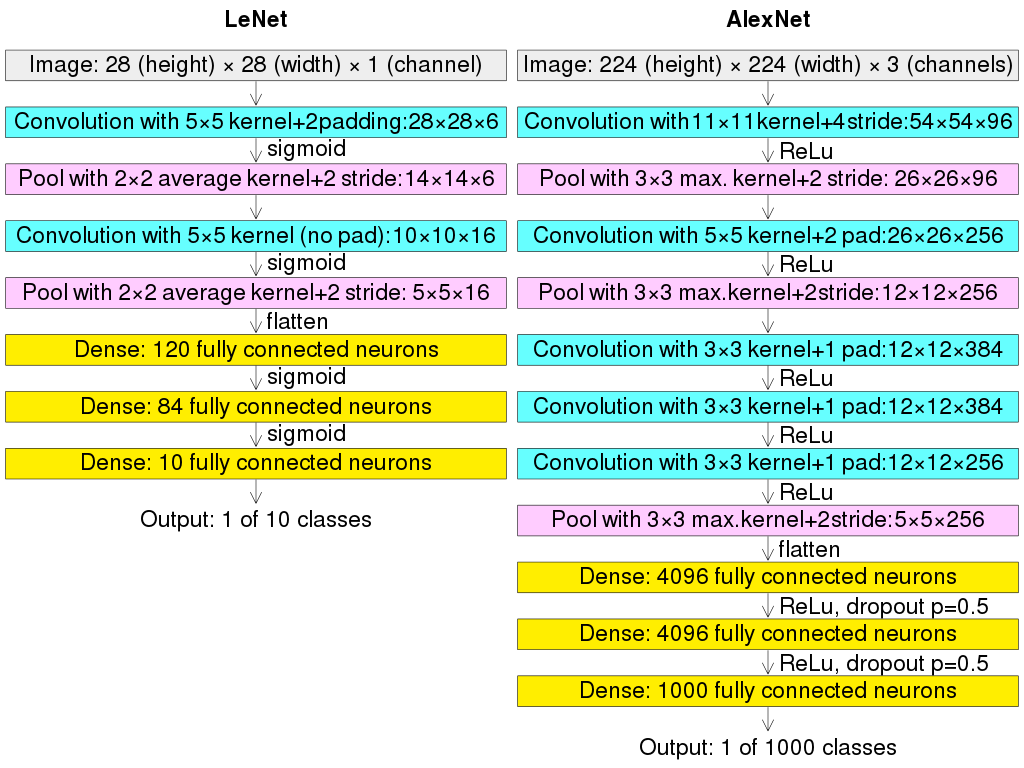
\includegraphics[width=0.8\textwidth]{Images/ANNArchitectures/lenet_vs_alexnet.png}
        \decoRule
        \caption[Comparing LeNet-5 and AlexNet]{Comparing the LeNet and AlexNet architectures: \href{https://en.wikipedia.org/wiki/AlexNet\#/media/File:Comparison_image_neural_networks.svg}{URL}.}
        \label{fig:Lenet_Alexnet_Comparison}
\end{figure}

\subsection{ResNet}
An ANN known as a residual neural network is distinguished by its shortcut connections that skip several layers. In this manner, it is possible to build ANNs that have hundreds of layers and are very deep without experiencing the vanishing gradients phenomenon. Additionally, it reduces the accuracy saturation issue, in which adding additional layers to a complex model causes the training error to increase.
\begin{figure}[H]
    \centering
        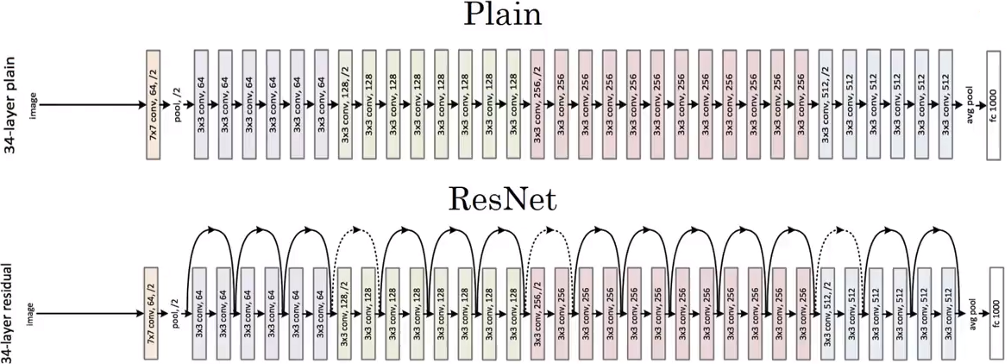
\includegraphics[width=1\textwidth]{Images/ANNArchitectures/resnet_vs_plain.png}
        \decoRule
        \caption[Comparing ResNet and plain architectures]{Comparing a ResNet and a plain model: \href{https://towardsdatascience.com/review-resnet-winner-of-ilsvrc-2015-image-classification-localization-detection-e39402bfa5d8}{URL}.}
        \label{fig:ResNet_Plain_Comparison}
\end{figure}

\subsection{Inception Module}
In CNNs, the appropriate size of the filters depends on how the important information is located in the training data. Filters with small kernels are better in detecting information with a local distribution, while large kernels are preferred when dealing with a global distribution. Each sample may have a different distribution, making it challenging to select an ideal filter.
\begin{figure}[H]
    \centering
        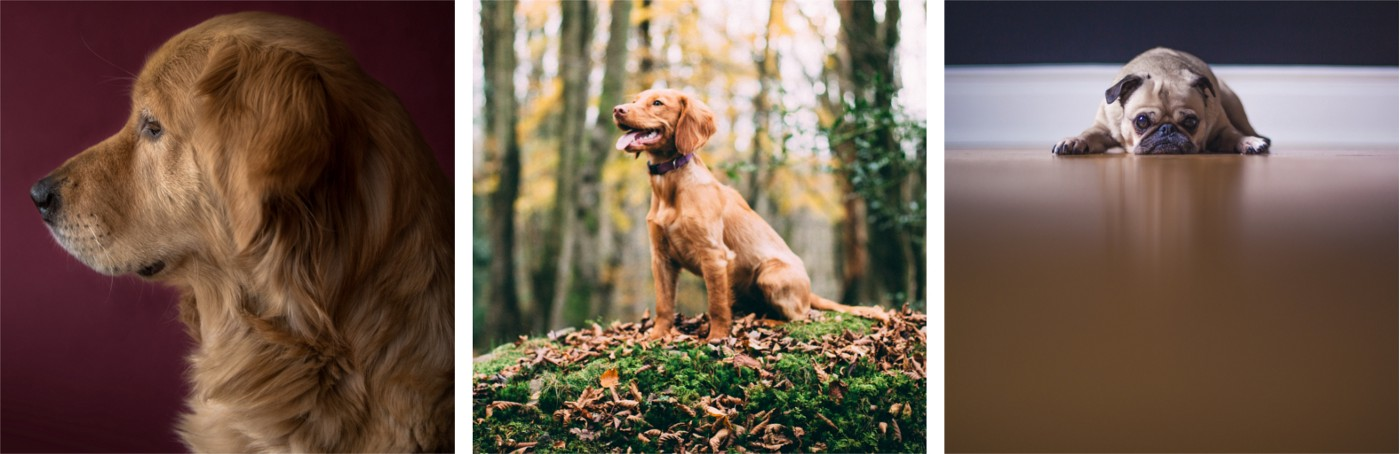
\includegraphics[width=0.8\textwidth]{Images/dogs_inception.jpg}
        \decoRule
        \caption[Variety of distribution of information.]{The dog, which is the important information, can occupy differently sized portions of the picture: \href{https://towardsdatascience.com/a-simple-guide-to-the-versions-of-the-inception-network-7fc52b863202}{URL}.}
        \label{fig:dogs_inception}
\end{figure}

The inception module \cite{inception_module} addresses this issue by providing multiple filters of various sizes that operate in parallel. These filters seek after the same information but in differently sized parts of the input. Consolidating their outputs is sufficient to determine whether one of them found the sought-after information because the one who identified it will overshadow the rest.

In its original form, it consists of three convolutional layers, with sizes of \(1\times1\), \(3\times3\), \(5\times5\), as well as one \(1\times1\) max pooling layer. To reduce computation, prior to the \(3\times3\), \(5\times5\) convolutions, and after the max pooling, additional \(1\times1\) convolutionals are added. These layers are dual-purposed, as they apply dimension reduction and an extra layer of ReLU activations.

\begin{figure}[H]
    \centering
        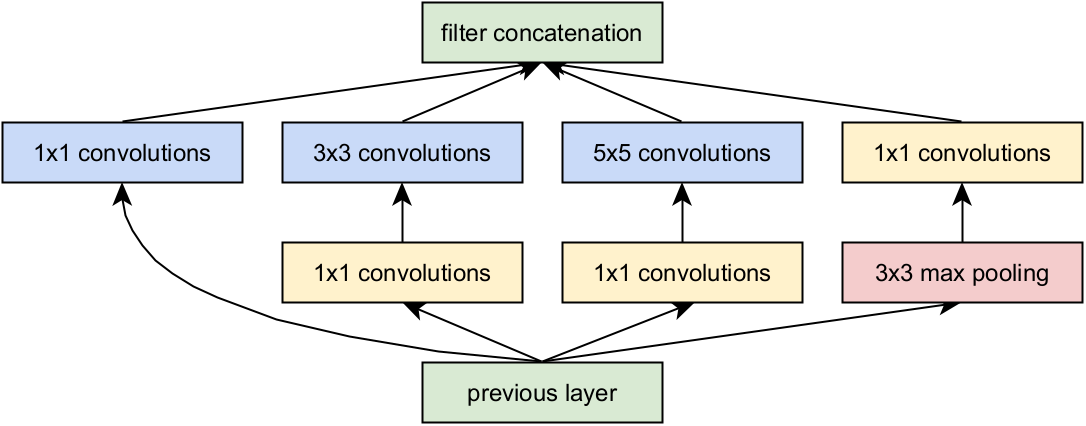
\includegraphics[width=0.8\textwidth]{Images/ANNArchitectures/inception_module.png}
        \decoRule
        \caption[Inception Module]{Architecture of the Inception module with dimension reductions.: \href{https://arxiv.org/abs/1409.4842}{URL}.}
        \label{fig:inception}
\end{figure}

\section{Federated Learning Algorithms}
\subsection{Distributed SGD}
Due to their iterative structure, conventional learning algorithms like SGD are inherently serial. Parallelism can only be applied over an example, e.g. pixels in a CNN, or over a mini-batch, where each example in it can be used in parallel. Synchronous SGD \cite{parallel_SGD}, a variation of mini-batch SGD, aims to enable cross-batch parallelism to reduce training time.

Before training starts, the dataset is distributed between \(N\) workers. In every iteration, each worker processes a mini-batch independently of the others, as follows:
\begin{itemize}
    \item it fetches the up-to-date model parameters;
    \item it then computes new parameters\footnote{Instead of parameters, it can calculate and send gradients, letting the synchronization service do the backpropagation. This is true for most distributed or federated algorithms.} using a local mini-batch;
    \item finally, these parameters are sent to a synchronization service, generally a chief thread\footnote{As the workers are usually in a shared memory environment, this can also be done by one of them.}, that computes the new model parameters. When this is done, a new iteration begins.
\end{itemize}

\begin{algorithm}[H]
    \caption[Distributed SGD]{\texttt{Distributed SGD.} The \(N\) workers are indexed by \(n\); \(B\) is the local mini-batch size, \(w\) are the model weights, and \(\eta\) is the learning rate.}
    \label{alg:Distributed_SGD}
    \begin{algorithmic}
        \Function {\textbf{Synchronization service executes:}}{}
            \State initialize $w_0$
            \State $D_{1 \ldots N} \gets$ (distribute data to $N$ workers)
            \For {each round $t = 1,2,\ldots$}
                \For {each worker $n \in N$ \textbf{in parallel}}
                    \State $w_{t+1}^n \gets$ WorkerUpdate($n,w_t$)
                \EndFor
                \State $w_{t+1} \gets \frac{1}{N} \sum_{n=1}^{N} w_{t+1}^n$
            \EndFor
        \EndFunction
        
        \Function {\textbf{WorkerUpdate}}{$n,w$} //Run on worker n
            \State $b \gets $ ($1$ batch of size $B$ from dataset $D_{n}$)
            \State $w \gets w - \eta \nabla l(w;b)$
            \State return $w$ to synchronization service
        \EndFunction
    \end{algorithmic}
\end{algorithm}

While initially intended for training in datacenters or localized clusters, it can easily be generalized for the federated setting by swapping out the workers for clients, the synchronization service with a server, and the distributed datasets with client generated ones. As a result, it became a major source of inspiration for FL.

\subsection{FederatedAveraging}
Many successful implementation of DL have relied on variations of SGD for optimization. As a matter of fact, they can be regarded as adaptations of the models and their loss functions to be more susceptible to optimization through simple gradient-based methods. Thus, it is natural that building FL algorithms begins with SGD.

Distributed SGD could naively be used in the federated setting, with each client computing the gradients of a single batch, a few samples, for each communication round. Although this method may be computationally efficient, it takes tens of thousands of training rounds to converge in a solution. This is prohibitive in a federated setting as communication costs are much higher than in a datacenter.

A straightforward method to reduce communication is expanding the batch until it includes the client's whole dataset. Thus, every client performs one full-batch (non-stochastic) gradient descent calculation per round. Furthermore, each client may have a different amount of examples, since in the federated setting, they are independently generated by the clients instead of being distributed by the server. As such, aggregation is weighted by the number of examples in each client. This approach is typically called FederatedSGD. 


While FederatedSGD improves the computation-to-communication ratio, a number of other problems emerge. First of all, clients might not be able to meet the very high memory requirements of full-batch gradient descent. Furthermore, when under non-iid data distribution, convergence of the global model is not guaranteed due to high divergence between the local models. A more sophisticated approach, that overcomes these issues, is maintaining a more balanced batch size while performing several updates to the local models before sharing them with the server. This method is referred as FederatedAveraging (FedAvg) \cite{FL-original-paper} and is the cornerstone of FL, as most FL algorithms are its derivatives.

\begin{algorithm}[H]
    \caption[FederatedAveraging]{\texttt{FederatedAveraging.} The \(N\) client are indexed by \(n\); k is the size of the local datasets, while K is their total size; E is the number of local epochs, \(B\) is the local mini-batch size, \(w\) are the model weights, and \(\eta\) is the learning rate.}
    \label{alg:FederatedAveraging}
    \begin{algorithmic}
        \Function {\textbf{Server executes:}}{}
            \State initialize $w_0$
            \For {each round $t = 1,2,\ldots$}
                \State $S_{t} \gets$ (set of selected clients)
                \For {each client $n \in S_{t}$ \textbf{in parallel}}
                    \State $w_{t+1}^n \gets$ ClientUpdate($n,w_t$)
                \EndFor
                \State $w_{t+1} \gets \sum_{n=1}^{N} \frac{k_n}{K} w_{t+1}^n$
            \EndFor
        \EndFunction
        
        \Function {\textbf{ClientUpdate}}{$n,w$}\textbf{:} //Run on client n
            \State $S_b \gets $ (split local dataset into batches of size $B$)
            \For {each local epoch $i$ from $i$ to $E$}
                \For {each $b \in S_b$}
                    \State $w \gets w - \eta \nabla l(w;b)$
                \EndFor
            \EndFor
            \State return $w$ to server
        \EndFunction
    \end{algorithmic}
\end{algorithm}

fedavg algorithm

\section{The FPGA Perspective}
\section{Thesis Approach}
